\documentclass[../main/report.tex]{subfiles}
\begin{document}

\chapter{Testing}

Does it work?

\section{VHDL system integration tests}

\subsection{Memory stores and kernel parameterization}

To verify that memory stores, as well as constant memory actually works, a simple kernel to fill the screen with a given color from constant memory was written.
This thereby also tests kernel parameterization, that is changing kernel behaviour with constants loaded at runtime.

\begin{figure}[H]
  \begin{code}
    ldc $data, 0       # Load the color green
    mv $address_hi, $id_hi
    mv $address_lo, $id_lo
    sw
    thread_finished
  \end{code}
  \caption{Kernel to test constant memory and parameterization}
  \label{fig:test-kernel-parameterization}
\end{figure}

Expected behaviour of test:
\begin{enumerate}
  \item
    The color green should successfully be loaded from constant memory.
  \item
    It should be stored to memory.
  \item
    The screen should be filled with the color green.
\end{enumerate}

\subsubsection*{simulation results}

\begin{figure}[H]
  \centering
  \begin{subfigure}[b]{\textwidth}
    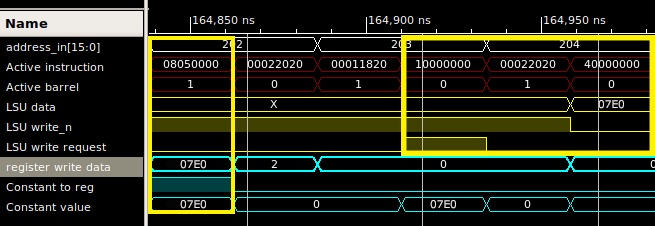
\includegraphics[width=\textwidth]{assets/Constant_load_&_store.png}
    \caption{Isim simulation of fillscreen @ 2 cores \& 2 barrels}
    \label{fig:isim-kernel-parameterization}
  \end{subfigure}
  \begin{subfigure}[b]{0.3\textwidth}
    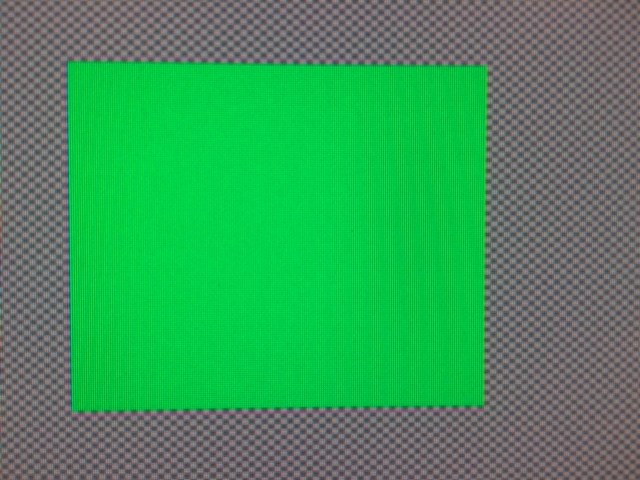
\includegraphics[width=\textwidth]{assets/green_screen.jpg}
    \caption{LX16 run of fillscreen}
    \label{fig:LX16-kernel-parameterization}
  \end{subfigure}
  \caption{Results from simulation and LX16}
\end{figure}

In the left yellow square of figure \ref{fig:isim-kernel-parameterization}, one can see the load constant instruction being executed (0x08050000) in barrel line 1.
The Constant to reg signal is asserted, and the constant value 0x07E0 is passed into the register write data signal.

In the right yellow square, the store word instruction (0x100000000) executes in barrel line 0.
The LSU accepts the write request same cycle (LSU write request goes high), and two cycles later the request packet reaches the LSU data line.
The LSU deasserts LSU write\_n, as the signal is active low, and the external ram handles the store request.

The value has now been successfuly written to memory, as can be verified in figure \ref{fig:LX16-kernel-parameterization}.

\subsection{Loads from primary memory}

\subsection{Instruction masking}

\subsection{Kernel square}




\subfile{../testing/io_testing.tex}


\section{PCB tests}

After receiving the finished PCB and the components, we performed the following tests before reaching a final (hardware-wise)functional computer.   

\subsection{Solder, signal and power test}
The puropse of these tests was to solder components and checking that their connections held, as well as checking that power correctly propagated through the board.  
\subfile{../testing/Solder_test.tex}

\subsection{Oscillator and clock test}
These tests consisted of using an oscilloscope in order to probe the outputs of the FPGA's oscillator and the high frequency and low frequency crystals.
\subfile{../testing/oscillation_test.tex}

\subsection{JTAG test}
In these tests we attempted to connect to respectively, the FPGA and the MCU by way of the appropriate headers, thereby verifying that they had been properly soldered in place and were functional.
\subfile{../testing/JTAG_test.tex}

\end{document}
